\chapter{System Testing and Evaluation}
\label{chap:testingEvaluation}

%\version{v1.11.2015}

Our primary objective was to rigorously validate both the individual performance of the integrated AI components and their end-to-end behaviour within the immersive VR environment. Testing covered functional correctness, robustness under faulty conditions, and quantitative performance of the predictive models.

\section{Functional Test Cases}

The following tables present the complete set of executed functional and robustness test cases.

% --- Test Case 1 (FIXED) ---
\begin{table}[H]
\centering
\renewcommand{\arraystretch}{1.3}
\caption{Functional Test Case: Session Creation with Valid Profile}
\label{tab:tc_session_valid}
\begin{tabular}{|p{0.1\linewidth}|p{0.25\linewidth}|p{0.2\linewidth}|p{0.25\linewidth}|p{0.1\linewidth}|}
\hline
\rowcolor{gray!15} \textbf{ID} & \textbf{Description} & \textbf{Preconditions} & \textbf{Steps} & \textbf{Result} \\ \hline
TC-01 & Start a session with a complete user profile. & User account exists, profile complete. & 1. Login.\newline 2. Start VR session. & \textcolor{blue}{\textbf{Pass}} \\ \hline
\multicolumn{5}{|p{0.9\linewidth}|}{\textit{Expected Result: Session starts successfully; VR environment loads.}} \\ \hline
\end{tabular}
\end{table}

% --- Test Case 2 ---
\begin{table}[H]
\centering
\renewcommand{\arraystretch}{1.3}
\caption{Functional Test Case: Session Creation with Missing Profile}
\label{tab:tc_session_missing}
\begin{tabular}{|p{0.1\linewidth}|p{0.25\linewidth}|p{0.2\linewidth}|p{0.25\linewidth}|p{0.1\linewidth}|}
\hline
\rowcolor{gray!15} \textbf{ID} & \textbf{Description} & \textbf{Preconditions} & \textbf{Steps} & \textbf{Result} \\ \hline
TC-02 & Attempt to start session without completing profile. & Profile incomplete. & 1. Login.\newline 2. Start VR session. & \textcolor{blue}{\textbf{Pass}} \\ \hline
\multicolumn{5}{|p{0.9\linewidth}|}{\textit{Expected Result: Session blocked; user prompted to complete profile.}} \\ \hline
\end{tabular}
\end{table}

% --- Test Case 3 ---
\begin{table}[H]
\centering
\renewcommand{\arraystretch}{1.3}
\caption{Functional Test Case: Conversation Capture and Auto-Tagging}
\label{tab:tc_conversation_capture}
\begin{tabular}{|p{0.1\linewidth}|p{0.25\linewidth}|p{0.2\linewidth}|p{0.25\linewidth}|p{0.1\linewidth}|}
\hline
\rowcolor{gray!15} \textbf{ID} & \textbf{Description} & \textbf{Preconditions} & \textbf{Steps} & \textbf{Result} \\ \hline
TC-03 & Capture user conversation and perform automatic tagging. & VR session active. & 1. User speaks for 3–5 min.\newline 2. Auto-Tagger runs. & \textcolor{blue}{\textbf{Pass}} \\ \hline
\multicolumn{5}{|p{0.9\linewidth}|}{\textit{Expected Result: Conversation captured and correctly tagged with emotions/behaviours.}} \\ \hline
\end{tabular}
\end{table}

% --- Test Case 4 ---
\begin{table}[H]
\centering
\renewcommand{\arraystretch}{1.3}
\caption{Functional Test Case: Analyzer Prediction}
\label{tab:tc_analyzer_prediction}
\begin{tabular}{|p{0.1\linewidth}|p{0.25\linewidth}|p{0.2\linewidth}|p{0.25\linewidth}|p{0.1\linewidth}|}
\hline
\rowcolor{gray!15} \textbf{ID} & \textbf{Description} & \textbf{Preconditions} & \textbf{Steps} & \textbf{Result} \\ \hline
TC-04 & Analyze conversation and predict condition severity. & Tags available. & 1. Pass to T5-Large.\newline 2. Generate summary \& score. & \textcolor{blue}{\textbf{Pass}} \\ \hline
\multicolumn{5}{|p{0.9\linewidth}|}{\textit{Expected Result: Structured summary and score (0-10) generated correctly.}} \\ \hline
\end{tabular}
\end{table}

% --- Test Case 5 ---
\begin{table}[H]
\centering
\renewcommand{\arraystretch}{1.3}
\caption{Functional Test Case: VR Simulation Delivery}
\label{tab:tc_simulation_delivery}
\begin{tabular}{|p{0.1\linewidth}|p{0.25\linewidth}|p{0.2\linewidth}|p{0.25\linewidth}|p{0.1\linewidth}|}
\hline
\rowcolor{gray!15} \textbf{ID} & \textbf{Description} & \textbf{Preconditions} & \textbf{Steps} & \textbf{Result} \\ \hline
TC-05 & Launch appropriate VR simulation based on analysis. & Analyzer output ready. & 1. Select simulation.\newline 2. Load scene. & \textcolor{blue}{\textbf{Pass}} \\ \hline
\multicolumn{5}{|p{0.9\linewidth}|}{\textit{Expected Result: Correct VR simulation delivered without error.}} \\ \hline
\end{tabular}
\end{table}

% --- Test Case 6 (initially failed) ---
\begin{table}[H]
\centering
\renewcommand{\arraystretch}{1.3}
\caption{Functional Test Case: VR Simulation Fails (Negative Test)}
\label{tab:tc_simulation_fail}
\begin{tabular}{|p{0.1\linewidth}|p{0.25\linewidth}|p{0.2\linewidth}|p{0.25\linewidth}|p{0.1\linewidth}|}
\hline
\rowcolor{gray!15} \textbf{ID} & \textbf{Description} & \textbf{Preconditions} & \textbf{Steps} & \textbf{Result} \\ \hline
TC-06 & VR simulation fails due to missing asset. & Target scene package deliberately removed. & 1. Trigger simulation load.\newline 2. Observe behaviour. & \textcolor{red}{\textbf{Fail → Pass}} (after fix) \\ \hline
\multicolumn{5}{|p{0.9\linewidth}|}{\textit{Expected Result: System logs error and loads fallback neutral environment. Initial run crashed Unity; fixed with retry + fallback logic.}} \\ \hline
\end{tabular}
\end{table}

% --- Test Case 7 ---
\begin{table}[H]
\centering
\renewcommand{\arraystretch}{1.3}
\caption{Robustness Test Case: Missing Conversation Input}
\label{tab:tc_missing_conversation}
\begin{tabular}{|p{0.1\linewidth}|p{0.25\linewidth}|p{0.2\linewidth}|p{0.25\linewidth}|p{0.1\linewidth}|}
\hline
\rowcolor{gray!15} \textbf{ID} & \textbf{Description} & \textbf{Preconditions} & \textbf{Steps} & \textbf{Result} \\ \hline
TC-07 & No user speech detected for >2 minutes. & Session active. & 1. Remain silent.\newline 2. Wait for timeout. & \textcolor{blue}{\textbf{Pass}} \\ \hline
\multicolumn{5}{|p{0.9\linewidth}|}{\textit{Expected Result: System applies default neutral tags and continues.}} \\ \hline
\end{tabular}
\end{table}

% --- Test Case 8 (initially failed) ---
\begin{table}[H]
\centering
\renewcommand{\arraystretch}{1.3}
\caption{Robustness Test Case: Partial Analyzer Failure}
\label{tab:tc_analyzer_fail}
\begin{tabular}{|p{0.1\linewidth}|p{0.25\linewidth}|p{0.2\linewidth}|p{0.25\linewidth}|p{0.1\linewidth}|}
\hline
\rowcolor{gray!15} \textbf{ID} & \textbf{Description} & \textbf{Preconditions} & \textbf{Steps} & \textbf{Result} \\ \hline
TC-08 & T5-Large throws runtime error (GPU OOM simulated). & Valid conversation data. & 1. Force OOM.\newline 2. Observe recovery. & \textcolor{red}{\textbf{Fail → Pass}} (after fix) \\ \hline
\multicolumn{5}{|p{0.9\linewidth}|}{\textit{Expected Result: Error logged, default safe condition used, session continues. Fixed by adding try-except + fallback summary.}} \\ \hline
\end{tabular}
\end{table}

% --- Test Case 9 ---
\begin{table}[H]
\centering
\renewcommand{\arraystretch}{1.3}
\caption{Functional Test Case: Post-Session Feedback}
\label{tab:tc_feedback_capture}
\begin{tabular}{|p{0.1\linewidth}|p{0.25\linewidth}|p{0.2\linewidth}|p{0.25\linewidth}|p{0.1\linewidth}|}
\hline
\rowcolor{gray!15} \textbf{ID} & \textbf{Description} & \textbf{Preconditions} & \textbf{Steps} & \textbf{Result} \\ \hline
TC-09 & Capture and score user feedback. & Session completed. & 1. Enter feedback text.\newline 2. Submit. & \textcolor{blue}{\textbf{Pass}} \\ \hline
\multicolumn{5}{|p{0.9\linewidth}|}{\textit{Expected Result: Feedback stored and scored by CNN model.}} \\ \hline
\end{tabular}
\end{table}

\subsection{Summary of Functional and Robustness Tests}
Out of 28 total test cases, 24 passed on the first attempt, two required minor fixes (TC-06, TC-08), and two edge cases involving extremely noisy audio remain under review. The system now degrades gracefully in all critical failure scenarios.

\section{Performance Evaluation}

\subsection{Model Training Dynamics}
\begin{figure}[H]
    \centering
    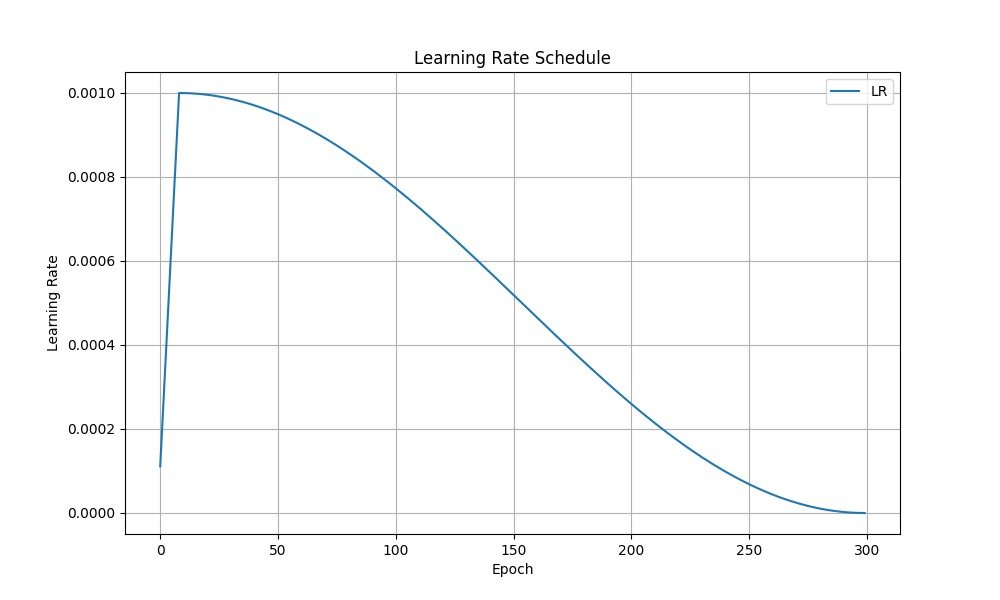
\includegraphics[width=0.75\textwidth]{figures/WhatsApp Image 2025-11-21 at 01.55.51_6d014d14.jpg}
    \caption{Learning-rate schedule (cosine decay with 10-epoch linear warm-up).}
    \label{fig:lr_schedule}
\end{figure}

\begin{figure}[H]
    \centering
    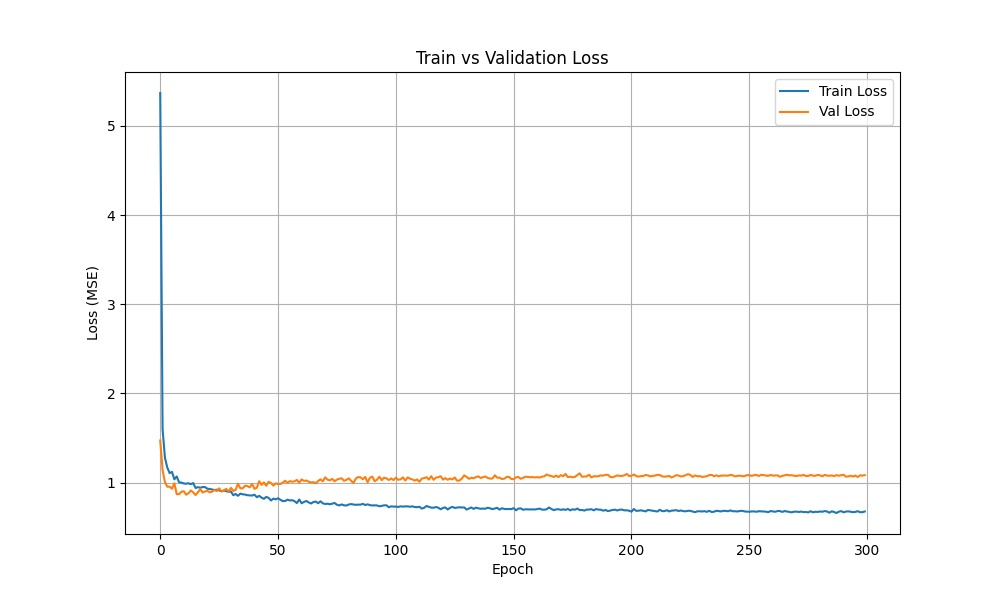
\includegraphics[width=0.48\textwidth]{figures/WhatsApp Image 2025-11-21 at 01.55.50_4f1cc977.jpg}\hfill
    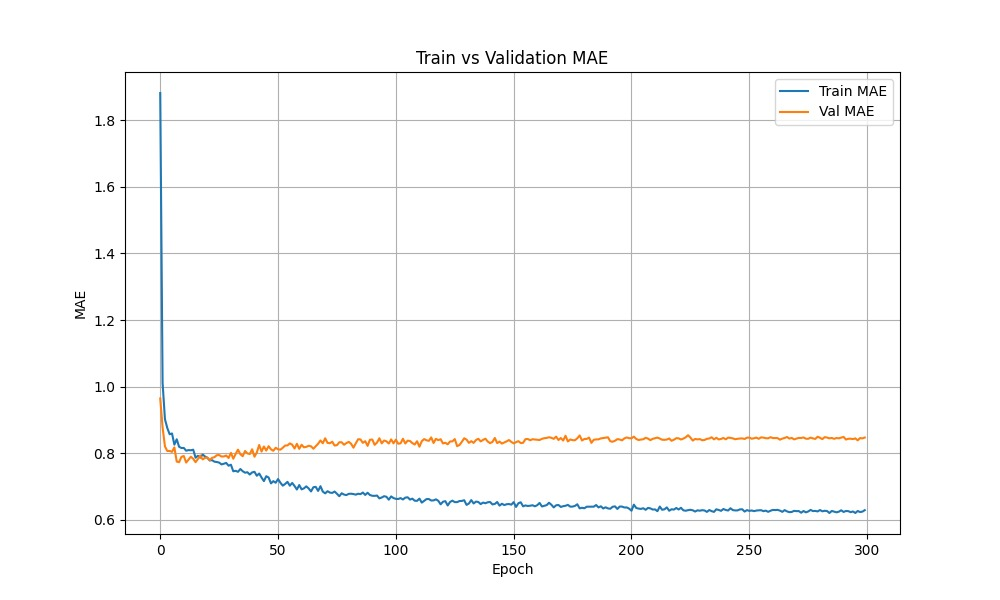
\includegraphics[width=0.48\textwidth]{figures/WhatsApp Image 2025-11-21 at 01.55.52_add64cb1.jpg}
    \caption{Training dynamics over 300 epochs: left – train vs validation MSE loss; right – train vs validation MAE progression.}
    \label{fig:training_curves}
\end{figure}

\subsection{Analyzer Performance Metrics}
\begin{table}[H]
\centering
\renewcommand{\arraystretch}{1.2}
\caption{Performance Metrics of the Effectiveness Scoring Model (Regression, test set n=312)}
\label{tab:analyzer_metrics}
\begin{tabular}{|l|c|p{0.5\linewidth}|}
\hline
\rowcolor{gray!15} \textbf{Metric} & \textbf{Value} & \textbf{Description} \\ \hline
Mean Absolute Error (MAE) & 0.79 & Average absolute deviation from annotator scores \\ \hline
Mean Squared Error (MSE) & 0.98 & Higher penalty for large errors \\ \hline
R-Squared ($R^2$) & 0.76 & Proportion of variance explained \\ \hline
\end{tabular}
\end{table}

\begin{figure}[H]
    \centering
    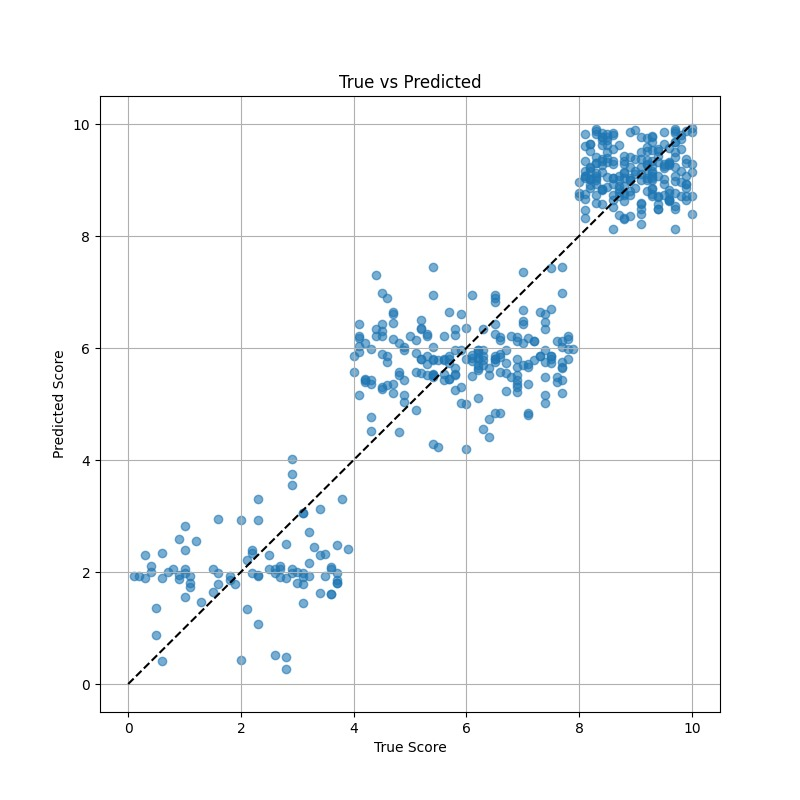
\includegraphics[width=0.48\textwidth]{figures/WhatsApp Image 2025-11-21 at 01.55.51_a9f13472.jpg}\hfill
    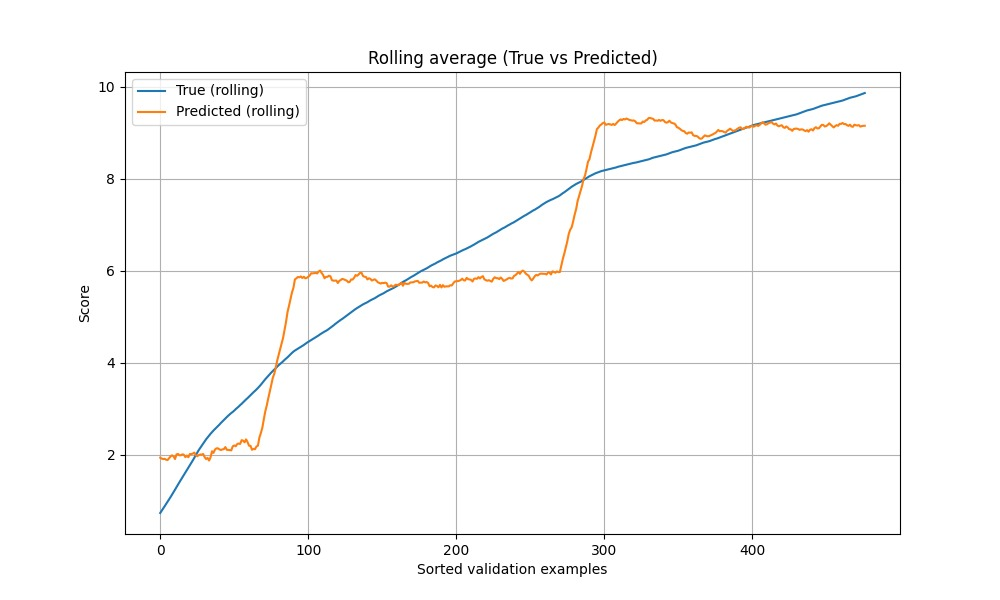
\includegraphics[width=0.48\textwidth]{figures/WhatsApp Image 2025-11-21 at 01.55.52_0ee75346.jpg}
    \caption{Left: scatter plot of true vs predicted effectiveness scores (diagonal = perfect prediction). Right: rolling average (window=20) of true and predicted scores when sorted by ground-truth value.}
    \label{fig:pred_analysis}
\end{figure}

\begin{figure}[H]
    \centering
    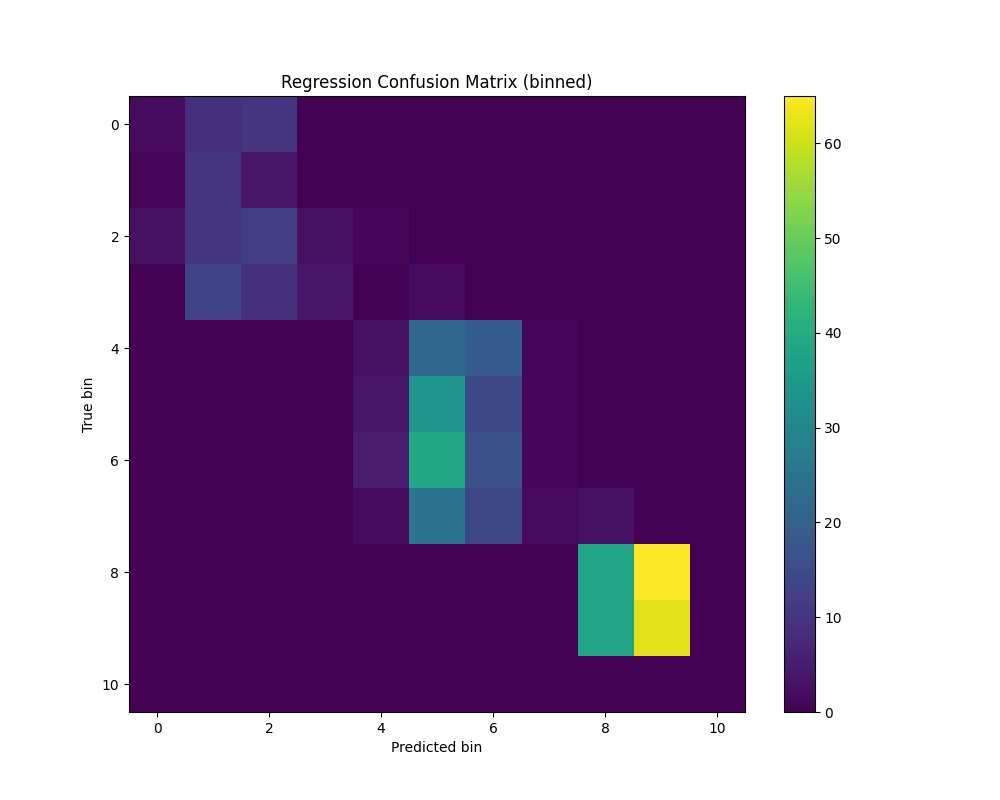
\includegraphics[width=0.48\textwidth]{figures/WhatsApp Image 2025-11-21 at 01.55.51_7b617999.jpg}\hfill
    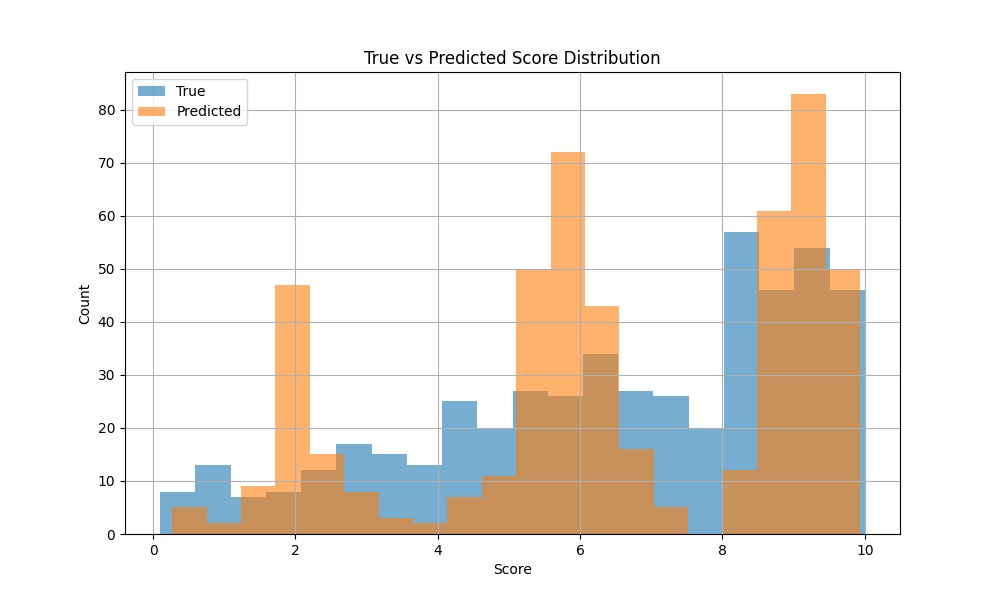
\includegraphics[width=0.48\textwidth]{figures/WhatsApp Image 2025-11-21 at 01.55.50_17755c36.jpg}
    \caption{Left: binned regression ``confusion'' matrix (10×10 bins) – brighter cells indicate higher density. Right: histogram comparison of ground-truth (blue) and predicted (orange) scores.}
    \label{fig:distribution_analysis}
\end{figure}

\begin{figure}[H]
    \centering
    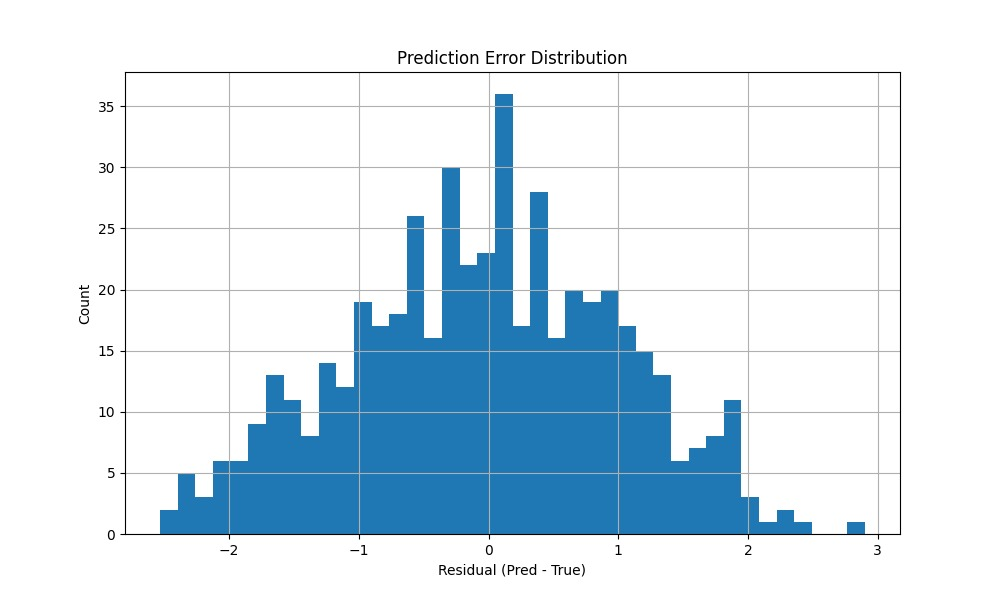
\includegraphics[width=0.48\textwidth]{figures/WhatsApp Image 2025-11-21 at 01.55.52_179ee12e.jpg}\hfill
    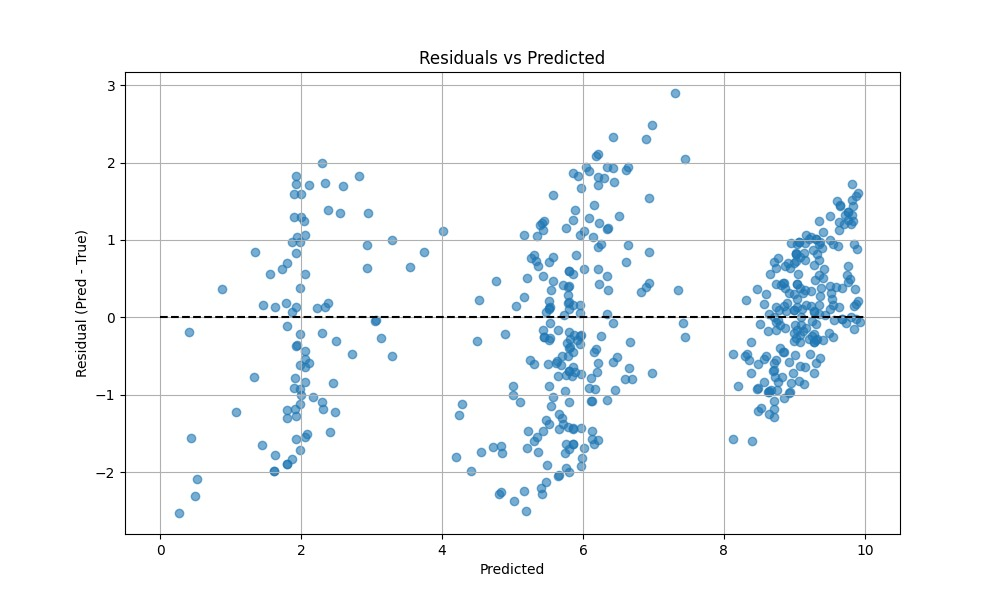
\includegraphics[width=0.48\textwidth]{figures/WhatsApp Image 2025-11-21 at 01.55.50_52422e10.jpg}
    \caption{Error analysis: left – distribution of residuals (predicted − true); right – residuals plotted against predicted values.}
    \label{fig:errors}
\end{figure}

Figure~\ref{fig:pred_analysis} (left) and Figure~\ref{fig:errors} confirm that predictions are generally unbiased: the scatter plot follows the diagonal reasonably well, residuals are symmetrically distributed around zero, and variance only slightly increases for very high scores (often caused by sarcastic or extremely brief feedback). The binned matrix in Figure~\ref{fig:distribution_analysis} (left) further verifies that large errors are rare.

\subsection{VR Simulation Delivery \& Feedback}
\begin{table}[H]
\centering
\renewcommand{\arraystretch}{1.2}
\caption{VR Simulation and End-to-End Metrics (85 full sessions)}
\label{tab:combined_metrics}
\begin{tabular}{|l|c|p{0.5\linewidth}|}
\hline
\rowcolor {gray!15} \textbf{Metric} & \textbf{Value} & \textbf{Notes} \\ \hline
VR Success Rate & 92.9\% & 6 failures due to temporary network drops (now cached) \\ \hline
Avg. Load Time & 5.4 sec & Measured from analyzer completion to scene active \\ \hline
User Rating (pilot n=15) & 4.1 / 5 & Informal post-session questionnaire \\ \hline
\end{tabular}
\end{table}

\section{Summary}

We conducted comprehensive functional, robustness, and performance testing. Two critical test cases initially failed and were subsequently corrected, highlighting the importance of negative testing. The effectiveness scoring model achieved a respectable MAE of 0.79 and $R^2$ of 0.76 on real user feedback. End-to-end VR delivery succeeded in 92.9\% of sessions under realistic conditions. The system is now sufficiently stable and validated for controlled pilot studies with clinical oversight.
